\documentclass{beamer}

\mode<presentation>
{
  \usetheme{Madrid}      % or try Darmstadt, Madrid, Warsaw, ...
  \usecolortheme{whale} % or try albatross, beaver, crane, ...
  \usefonttheme{serif}  % or try serif, structurebold, ...
  \setbeamertemplate{navigation symbols}{}
  \setbeamertemplate{caption}[numbered]
  \setbeamercovered{dynamic}
} 
\usepackage{amsmath}
\usepackage{amssymb}
\usepackage[utf8]{inputenc}
\usepackage[T1]{fontenc}
\usepackage{stmaryrd}
\usepackage[all]{xy}
\usepackage{graphicx}

\usepackage{relsize}
\usepackage[bbgreekl]{mathbbol}
\usepackage{amsfonts}
\DeclareSymbolFontAlphabet{\mathbb}{AMSb}
\DeclareSymbolFontAlphabet{\mathbbl}{bbold}
\newcommand{\Prism}{{\mathlarger{\mathbbl{\Delta}}}}

\theoremstyle{plain}
\newtheorem{proposition}{Proposition}[section]
\theoremstyle{definition}
\theoremstyle{remark}
\newcommand{\Q}{\mathbb{Q}}
\newcommand{\Z}{\mathbb{Z}}
\newcommand{\F}{\mathbb{F}}
\newcommand{\mo}{\mathcal{O}}

\title{Ribet-Herbrand Theorem}
\author{Anlun Li}
\institute{USTC}
\date{May 25, 2022}

\begin{document}
\begin{frame}
    \titlepage
\end{frame}

%Uncomment these lines for an automatically generated outline.
\begin{frame}{Plan}
    \begin{itemize}
        \item A Short Review
        \item Two Stronger Versions of The Theorem
        \item Introduction to the Modular Forms
        \item Ribet's Idea of the proof
    \end{itemize}
\end{frame}


\begin{frame}{Notations}
    Let  $A=Cl(\Q(\mu_p))$ finite ideal class group, $C=A/A^p$ is a $\F_p$ vector space.
    \vskip 0.2cm
    $ \Delta=Gal(\Q(\mu_p)/\Q) \stackrel{\sim}{\longrightarrow} (\Z/p\Z)^*$
    \vskip 0.2cm
    $G_{\Q}=Gal(\bar{\Q}/\Q)$ the absolute Galois group.
    \vskip 0.2cm
    $\chi: G_{\Q} \to Gal(\Q(\mu_p)/\Q) \stackrel{\sim}{\longrightarrow} (\Z/p\Z)^*$, sometimes it will also denote a Dirichlet character.
    \vskip 0.2cm
    $H=\{z\in \mathbb{C}:Im(Z)>0\}$, the upper half plane.

\end{frame}
\iffalse
\begin{frame}{Kummer's Result}
    Kummer proved that:
    \begin{proposition}[Kummer]
        $p \mid h_K \ \iff \exists$ positive even integer r, such that
        $p \mid \zeta(1-r)$
    \end{proposition}
    We may be interested in a more explicite description.
\end{frame}
\fi
\begin{frame}{Decomposition}
    \begin{lemma}[Decomposition Lemma]
        If R is a commutative ring containing $\{ \langle \mu_n \rangle \}$ and $\frac{1}{n}$,
        G is an abelian group with order n, then for $R[G]$ -module M, we have
        \[ M= \bigoplus_{\chi}M(\chi), \]
        where $M(\chi)=\{m\in M: \sigma m =\chi(\sigma) m \ \text{for every } \sigma \in G\} $, $\chi$
        is a Dirichlet character modulo n.
    \end{lemma}\pause
    View $C$ as $\mathbb{F}_p[Gal(K/\Q)]$ module, we have:
    \[ C=\bigoplus_{i=1}^{p-1} C(\chi^{i}), \]
    as a $\mathbb{F}_p$ vector space.

\end{frame}

\begin{frame}{Statements of the Theorem}
    Let $\frac{t}{e^t-1}=\sum_{n=0}^{\infty}B_k\frac{t^n}{n!}$. $B_n$ is called Bernoulli numbers.
    A fact states that $\zeta(1-n)=-\frac{B_n}{n}$ for $n \ge 1$.\pause
    \vskip 0.2cm
    In the 1930s, Herbrand found:
    \begin{proposition}[Herbrand,1930s]
        Let k $\in [2,p-3] $ be an even integer. If $C(\chi^{1-k}) \ne 0$, then $p |B_k$.
    \end{proposition}
    This is a consequence of the Stickelberger's Theorem.

    Today, we mainly focus on the converse.
    \begin{theorem}[Ribet,1970s]
        Let k $\in [2,p-3] $ be an even integer. If $p|B_k$, then $C(\chi^{1-k}) \ne 0.$
    \end{theorem}
\end{frame}

\section{Stronger versions}
\begin{frame}{Version 2}
    We first introduce two stronger versions of the theorem.
    \begin{theorem}
        Let k $\in [2,p-3] $ be an even integer, and suppose that $p|B_k$.
        Then there exists a galoisian extension $E/\Q$ containing $K=\Q(\mu_p)$ such that
        \begin{itemize}
            \item The extension $E/K$ is everywhere unramified.
            \item The group $H=Gal(E/K)$ is a non-trivial p-elementary commutative group, i.e. $H \cong (\Z/p\Z)^n$.
            \item For every $\sigma \in $G=Gal(E/$\Q$), $\bar{\sigma} \in \Delta=Gal(K/\Q)$, and every $\tau \in H$,
                  \[\sigma \tau \sigma^{-1}= \chi(\bar{\sigma})^{1-k}. \tau \]
        \end{itemize}
    \end{theorem}
    This theorem indeed implies Ribet's Theorem.
\end{frame}

\begin{frame}{Version 3}
    Let $D  \subset G_{\Q}$ denote one of the decomposition group at the prime p, i.e.
    $D=\{\sigma \in G_{\Q}: \wp^{\sigma}=\wp, p \subset \wp \subset \bar{\Z} \}$. $\chi: G_{\Q} \to Gal(\Q({\mu_p})/\Q) \stackrel{\sim}{\longrightarrow} \mathbb{F}_p^*$.

    The following theorem is stronger than the previous one.
    \begin{theorem}
        Let k $\in [2,p-3] $ be an even integer, and suppose that $p|B_k$. There exists
        a finite extension $\F/\F_p$, and a continuous representation $\rho : G_{\Q} \to GL_2(\F)$, such that
        \begin{itemize}
            \item $\rho $ is \textbf{unramified} at every prime $l \ne p$.
            \item $ \rho \sim \begin{pmatrix}
                          1 & \gamma     \\
                            & \chi^{k-1}
                      \end{pmatrix}, \gamma: G_{\Q} \to \F \ \text{is non-trivial.} $
            \item $\rho |_{D}$ is semi-simple.
        \end{itemize}
    \end{theorem}
    Note that in such case, a representation is semi-simple if and only if its image cannot be divided by p.
\end{frame}

\section{Modular Forms}
\begin{frame}{Modular Forms}
    \begin{definition}[Congruence Group]
        $\Gamma$ is called a congruence group if there exists N, s.t. $\Gamma(N) \subset \Gamma$,
        where $\Gamma(N)=\{ \begin{pmatrix}
                a & b \\
                c & d
            \end{pmatrix} \in SL_2(\Z):\begin{pmatrix}
                a & b \\
                c & d
            \end{pmatrix} \equiv \begin{pmatrix}
                1 & 0 \\
                0 & 1
            \end{pmatrix} (mod \ N) \}$.
    \end{definition}
    We will also need the following definitions.
    \[\begin{matrix}
            \Gamma(N)      & = & \{\begin{pmatrix}
                a & b \\
                c & d
            \end{pmatrix}\in SL_2(\Z): \begin{pmatrix}
                a & b \\
                c & d
            \end{pmatrix} \equiv \begin{pmatrix}
                1 & 0 \\
                0 & 1
            \end{pmatrix} (mod \ N) \}   \\
            \bigtriangleup &   &                                                                                                                       \\
            \Gamma_1(N)    & = & \{\begin{pmatrix}
                a & b \\
                c & d
            \end{pmatrix}\in SL_2(\Z): \begin{pmatrix}
                a & b \\
                c & d
            \end{pmatrix} \equiv \begin{pmatrix}
                1 & * \\
                0 & 1
            \end{pmatrix} (mod \ N)   \} \\
            \bigtriangleup &   &                                                                                                                       \\
            \Gamma_0(N)    & = & \{ \begin{pmatrix}
                a & b \\
                c & d
            \end{pmatrix}\in SL_2(\Z): \begin{pmatrix}
                a & b \\
                c & d
            \end{pmatrix} \equiv \begin{pmatrix}
                * & * \\
                0 & *
            \end{pmatrix} (mod \ N)  \} \\
        \end{matrix}\]
\end{frame}

\begin{frame}{Modular Forms}
    \begin{definition}[Modular Curves]
        $Y(\Gamma):=\Gamma \setminus H=\{\Gamma \tau : \tau \in H \}$, is the set of orbits.

        $X(\Gamma):=\Gamma \setminus H^*$, where $H^*=H \cup P^1(\Q)$.
    \end{definition}
    Fact: $X(\Gamma)$ is a compact Riemann Surface.
    \begin{figure}
        \centering
        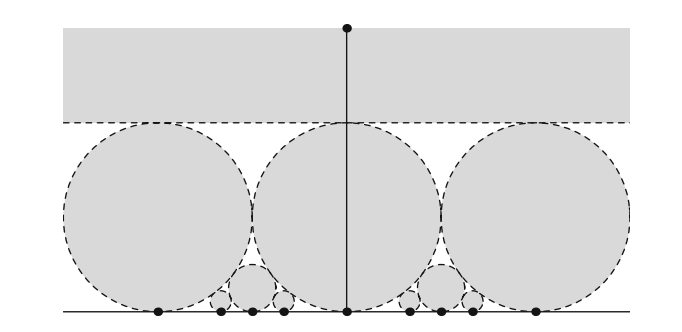
\includegraphics[scale=0.30]{fig2.5.png}
        \caption{Neighborhoods of $\infty$ and of some rational points}
    \end{figure}
\end{frame}

\begin{frame}{An Example:$X(SL_2(\Z)) \cong S^2$}
    \begin{figure}
        \centering
        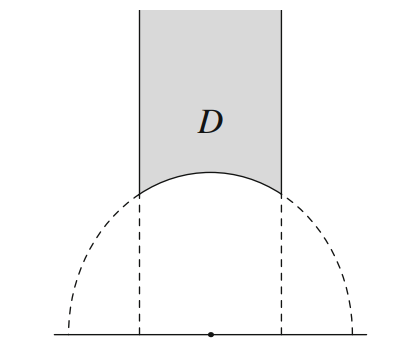
\includegraphics[scale=0.30]{the fundamental domain for SL_2(Z).png}
        \caption{the fundamental domain for $SL_2(\Z)$}
    \end{figure}
\end{frame}

\begin{frame}{Modular Forms}

    \begin{definition}[Modular Forms of weight k with respect to $\Gamma$]
        $f: H \to \mathbb{C} $ is called modular forms of weight k with respect to $\Gamma$
        (i.e. $f \in M_k(\Gamma)$) if:
        \begin{itemize}
            \item f is holomorphic in H
            \item $f[\gamma]_k=f$ for any $\gamma \in \Gamma$
            \item $f[\alpha]_k$ is holomorphic at $\infty$ for any $\alpha \in SL_2(\Z)$
        \end{itemize}
    \end{definition}
    \pause
    Moreover,
    if $a_0=0$ in $f[\alpha]_k$'s fourier expansion for all $\alpha \in SL_2(\Z)$,
    then f is called a \textbf{cusp form} of weight k respect to $\Gamma$, i.e. $f \in S_k(\Gamma)$.\pause
    \vskip 0.2cm
    If we replace "holomorphic" by \textbf{"meromorphic"}, then the set is $A_k(\Gamma)$, called \textbf{Automorphic form}.

\end{frame}

\begin{frame}{Modular Forms}
    \begin{proposition}[Decomposition of $M_k(\Gamma_1(N))$]
        \[M_k(\Gamma_1(N))=\bigoplus _{\chi } M_k(N,\chi),\] where $M_k(N,\chi)=\{f: f[\gamma]_k=\chi(d_{\gamma})f \  \text{for all} \ \gamma \in \Gamma_0(N) \}$,
        and $\chi$ is a Dirichlet character modulo N.
    \end{proposition}
    \begin{proof}
        Note that $\Gamma_0(N)/\Gamma_1(N) \cong (\Z/N\Z)^*$.
    \end{proof}
\end{frame}


\begin{frame}{Pic$^0$ and Jacobi}
    \begin{definition}
        $Pic^0(X)=Div^0(X)/Div^l(X)$
    \end{definition}\pause
    \begin{definition}
        $Jac(X)=\Omega^1_{hol}(X)^{\wedge} /H_1(X,\Z)$
    \end{definition}
    Note that the right side is a complex torus of dimension g. \pause
    \begin{theorem}[Abel Theorem]
        For X a compact Riemann Surface, if $g > 0$, then
        \[ Pic^0(X) \cong Jac(X),\  [\sum_x n_x x]  \mapsto \sum_x n_x\int_{x_0}^x \]
    \end{theorem}
\end{frame}

\begin{frame}{Maps induced by $\sigma: X \to Y$}
    Let $\sigma: X \to Y$ be a nonconstant holomorphic map between compact Riemann Surfaces, then we have
    forward map and reverse map of $Pic^0$.
    \[\sigma_*: Pic^0(X) \to Pic^0(Y)\]
    \[\sigma_*[\sum_x n_x x] = [\sum_x n_x \sigma(x)]\]
    \vskip 0.2cm
    \[\sigma^*: Pic^0(Y) \to Pic^0(X)\]
    \[\sigma^*[\sum_y n_y y] = [\sum_y n_y \sum_{x\in \sigma^{-1}y} e_x x] \]
\end{frame}

\begin{frame}{Modular Forms}
    \begin{theorem}
        Let k be an even positive integer, and $\Gamma$ be a congruence group of $SL_2(\Z)$.
        The following map is an isomorphism of complex vector space.
        \[ \omega: A_k(\Gamma) \to \Omega^{\otimes k/2}(X(\Gamma))\]
        In particular, $\omega$ induces an isomorphism from $S_2(\Gamma)$ to $\Omega_{hol}^1(X(\Gamma))$
    \end{theorem}
\end{frame}

\begin{frame}{Hecke Operators(1)}
    We can define two \textbf{Operators} from $M_k(\Gamma_1(N))$ to $ M_k(\Gamma_1(N))$.
    Let f be a modular form respect to $\Gamma_1(N)$, i.e. $f \in M_k(\Gamma_1(N))$.\pause
    \begin{definition}[$\langle n \rangle$]
        For $(n,N)=1$, define
        \[\langle d\rangle f=f[\alpha ]_k \ \text{for an } \alpha =\begin{pmatrix}
                a & b      \\
                c & \delta
            \end{pmatrix}\in \Gamma_0(N), \text{where} \ \delta \equiv  d \ \text{mod(N)}.\]
        For $(n,N)>1$, $\langle d\rangle f=0$.
    \end{definition}\pause
    Fact:
    \begin{itemize}
        \item $\langle d \rangle$ is independent of the choice of $\alpha$.
        \item $\langle d\rangle\langle e\rangle=\langle e\rangle\langle d\rangle=\langle de\rangle$.
        \item $M_k(N,\chi)=\{f: \langle d\rangle f=\chi(d)f \  \text{for all} \ d\in (\Z/N\Z)^* \}$
    \end{itemize}  
     
\end{frame}

\begin{frame}{Hecke Operators(2)}
    Let $\Gamma_1(N)\begin{pmatrix}
            1 & 0 \\
            0 & p
        \end{pmatrix}\Gamma_1(N)=\bigcup_j\Gamma_1(N) \beta_j, \ \text{for some}\  \beta_j(\in M_2(Z)) \equiv \begin{pmatrix}
            1 & * \\
            0 & p
        \end{pmatrix} (mod\  N), det \  \beta =p$.
    \begin{definition}[$T_p$]
        \[T_p f=f[\Gamma_1(N)\begin{pmatrix}
                1 & 0 \\
                0 & p
            \end{pmatrix}\Gamma_1(N)]:=\sum_jf[\beta_j]_k\]
        In general, $T_1=Id$, and $T_{p^r}=T_pT_{p^{r-1}}-p^{k-1}\langle p \rangle T_{p^{r-2}}, \text{for } r\ge2$.
        $T_{nm}=T_nT_m$ for $(n,m)=1$.
    \end{definition}
\end{frame}

\begin{frame}{Facts of Hecke Operators}
    We list serveral facts we will use.
    \begin{itemize}
        \item $T_m \langle n \rangle=\langle n \rangle T_m$
        \item T defines a map from $J_1(N)=Jac(X(\Gamma_1(N))) $ to itself, where T is $T_n$ or $\langle n \rangle$ for any $n \in \Z_{>0}$.
              %           \item Note T cannot be defined from $X(\Gamma_1(N))$ to itself.
    \end{itemize}
\end{frame}


\begin{frame}{Eigenform }
    \begin{definition}
        A non zero modular form f $\in M_k(\Gamma_1(N))$ is called an \textbf{eigenform} if it is an eigenform for the Hecke Operators $T_n$ and
        $\langle n \rangle$ for all $n \in \Z^+$. Moreover, if $a_1(f)=1$, then f is called a \textbf{normalized eigenform}.
    \end{definition}
    Since $M_k(N,\chi)=\{f: \langle d\rangle f=\chi(d)f \  \text{for all} \ d\in (\Z/N\Z)^* \}$,
    for every eigenform f, there exists a Dirichlet character $\chi$, $f\in M_k(N,\chi)$.

\end{frame}

\begin{frame}{Hecke algebra over $\Z$}
    \begin{definition}
        $T_{\Z}=\Z[\{T_n,\langle n \rangle:n \in \Z^+\}]$, the algebra of $S_2(\Gamma_1(N))$ generated over $\Z$.
    \end{definition}\pause
    \begin{proposition}
        $T_{\Z}$ is a finite generated $\Z$ module.
    \end{proposition}
    \begin{proof}
        $T_{\Z}$ can be viewed as a submodule of $End(H_1(X_1(N)),\Z)$.
    \end{proof}\pause
    \begin{corollary}
        Let f be a normalized eigenform, then $K_f=\Q(\{a_n(f)\})$ is a number field.
    \end{corollary}
    $d$ denotes the dimension of $K_f$ over $\Q$.
\end{frame}

\begin{frame}{Abelian Variety constructed by Shimura}
    Let f $\in S_2(\Gamma_1(N))$ be a newform at the level N and an eigenform of
    the Hecke algebra $T_{\Z}$. $J_1(N)=Jac(X_1(N))$.
    \[\lambda_f : T_{\Z} \to \mathbb{C}, Tf=\lambda_f(T)f\]
    and its kernel $I_f=ker(\lambda_f)=\{T\in T_{\Z}: Tf=0\}$.
    \begin{definition}
        The Abelian Variety associated to f is defined to be
        \[A_f=J_1(N)/I_fJ_1(N)\]
    \end{definition}
\end{frame}

\begin{frame}{A Property of $A_f=J_1(N)/I_fJ_1(N)$}
    Let $V_f= $ Span $(\{f^{\sigma}|\sigma: K_f \to \mathbb{C} \text{ is an embedding}\})$, a subspace of $S_2=S_2(\Gamma_1(N))$,
    $V_f^{\wedge}$ is its dual space $\subset S_2^{\wedge}$. $\Lambda_f=H_1(X_1(N),\Z)|_{V_f}$. It's natural to define
    \[J_1(N) \to V_f^{\wedge}/\Lambda_f, \quad [\varphi] \mapsto \varphi|_{V_f} +\Lambda_f \]
    \pause
    \begin{proposition}
        Let f $\in S_2(\Gamma_1(N))$ be an eigenform and newform with number field $K_f$, then
        \[A_f \cong V_f^{\wedge}/\Lambda_f, \quad [\varphi] + I_fJ_1(N) \mapsto \varphi|_{V_f} +\Lambda_f\]
    \end{proposition}
    The right side is a complex torus of dimension $[K_f:\Q]$.
\end{frame}

\begin{frame}{Igusa Theorem}
    Compact Riemann Surface is algebraic. But $X_0(N),X_1(N)$ can be taken as algebraic curves over $\Q$.
    \vskip 0.2cm
    Henceforce, $X_1(N)$ denotes the modular curve as a nonsingular algebraic curve over $\Q$.
    Let $\widetilde{X}_1(N)$ denote its reduction at $\mathbb{F}_p$.
    \begin{theorem}[Igusa Theorem]
        Let N be a positive number, and prime $p \nmid N$, then
        $X_1(N)$ acquires good reduction at p.
    \end{theorem}

\end{frame}

\begin{frame}{Eichler-Shimura Relation}
    \begin{theorem}[Eichler-Shimura Relation]
        Let p $\nmid $ N. The following diagram commutes.
        \[\xymatrix{\ar @{} [dr] |{}
            Pic^0(X_1(N)) \ar[d] \ar[r]^{T_p} & \quad \ Pic^0(X_1(N)) \ar[d] \\
            Pic^0(\widetilde{X}_1(N)) \ar[r]^{\sigma_{p,*}+\widetilde{\langle p \rangle}_*\sigma^*_p} & \quad  \ Pic^0(\widetilde{X}_1(N)) } \]
    \end{theorem}
    Here
    \begin{itemize}
        \item $\sigma_p([x_0,x_1,\cdots,x_n])=[x_0^p,x_1^p,\cdots,x_n^p]$
        \item $\sigma_{p,*}(Q)= \sigma_p(Q)$
        \item $\sigma_p^*(Q)=p \  \sigma_p^{-1}(Q)$
    \end{itemize}

\end{frame}
\section{Galois Representation}
\begin{frame}{l-adic Galois Representation}
    Since $X_1(N)$ is defined over $\Q$ , we can define a $G_{\Q}$ action on $Pic^0(X_1(N))$.

    For each n, there is a commutative diagram.
    \[\xymatrix{
            G_{\Q} \ar[d] \ar[rd] &\\
            Aut(Pic^0(X_1(N))[l^n])  &  Aut(Pic^0(X_1(N))[l^{n+1}]) \ar[l]
        }
    \]\pause
    We state without proof that the inclusion below is an isomorphism.
    \[i_n: Pic^0(X_1(N))[l^n] \hookrightarrow Pic^0(X_1(N)_{\mathbb{C}})[l^n]( \cong Jac[l^n] \cong (\Z/l^n\Z)^{2g})\]
    \pause
    So these induce a homomorphism
    \[ \rho_{X_1(N),l}: G_{\Q}\to GL_{2g}(\Z_l) \subset GL_{2g}(\Q_l)\]
\end{frame}

\begin{frame}{l-adic Galois Representation}
    \begin{theorem}
        Let l be prime and let N be a positive integer. The Galois representation
        $\rho_{X_1(N),l}$ is \textbf{unramified} at every prime $p \nmid lN$. For any such p,
        let $\wp \subset \bar{\Z}$ be any maximal ideal over p. Then $\rho_{X_1(N),l}(Frob_{\wp})$
        satisfies the polynomial equation.
        \[x^2-T_px+\langle p \rangle p=0\]
    \end{theorem}
\end{frame}

\begin{frame}{l-adic Galois Representation}
    Since $\ker(Pic^0(X_1(N))[l^n]\twoheadrightarrow  A_f[l^n])$ is stable unber $G_{\Q}$(we omit the proof), the following diagram commutes.
    \[\xymatrix{
        G_{\Q} \ar[d] \ar[rd] &\\
        Aut(Pic^0(X_1(N))[l^n]) \ar[d] &  Aut(Pic^0(X_1(N))[l^{n+1}]) \ar[l] \ar[d] \\
        Aut(A_f[l^n]) & Aut(A_f[l^{n+1}]) \ar[l]
        }
    \]
    And \[Ta_l(A_f) := \lim_{\leftarrow}A_f[l^n] \cong \lim_{\leftarrow} (\Z/l^n\Z)^{2d} \cong \lim_{\leftarrow}(\Z_l)^{2d}\]
\end{frame}

\begin{frame}{l-adic Galois Representation}
    As a corollary of the previous theorem, we have:
    \begin{theorem}
        Let f be a normalized, newform and eigenform in $S_2(N,\chi)$, \ $\rho_{A_f,l}: G_{\Q} \to GL_{2d}(\Q_l)$, is unramified at every prime $p \nmid lN$. And $\rho(Frob_{\wp})$ satisfies
        \[x^2-a_p(f)x+\chi(p)p=0\]
    \end{theorem}
%    We omit the proof that for such f, $T_pf=a_p(f)f$.
\end{frame}



\begin{frame}{l-adic Galois Representation}
    Let $V_l(A_f):=Ta_l(A_f) \otimes \Q \cong \Q_l^{2d}$
    \begin{lemma}
        $V_l(A_f)$ is a free $K_f \otimes_{\Q} \Q_l$-module of rank 2.
    \end{lemma}
    Using the canonical isomorphism
    $K_f \otimes \Q_l \cong \prod_{\lambda | l}K_{f,\lambda}$, we get
    \[\rho_{f,\lambda} : G_{\Q} \to GL(V_l(A_f)\otimes_{K_f \otimes \Q_l}K_{f,\lambda} ) \to GL_2(K_{f,\lambda})\]

\end{frame}

\begin{frame}{l-adic Galois Representation}
    Let f $\in S_2(N,\chi)$ be a normalized eigenform with number field $K_f$.
        Let l be a prime, for each maximal ideal $\lambda$ of $\mo_{K_f}$ lying over l,
        there is a 2-dimensional Galois representation
        \[\rho_{f,\lambda}: G_{\Q}\to GL_2(K_{f,\lambda}).\]
    As a corollary to the previous theorem, we get the following:
    \begin{theorem}
        This representation is unramified at every prime $p \nmid lN$. For any such
        p, let $\wp \subset \bar{\Z}$ be any maximal ideal lying over p. Then $\rho_{f,\lambda}(Frob_{\wp})$ satisfies
        the polynomial equation:
        \[x^2-a_p(f)x+\chi(p)p=0.\]
    \end{theorem}
\end{frame}


\section{Ribet's Idea}

\begin{frame}{Reduction}
    Let $L/\Q_p$ be a finite extension, $\mo$ the ring of intergers of L, $\pi$ the
    unique maximal ideal of $\mo$, and $\F= \mo / \pi$ the residue field.
    \vskip 0.2cm
    Let $\rho: G_{\Q} \to GL(V)$ be a continuous representation. Then there exists a $\mo$-lattice $\Lambda \subset V$,
    which is $G_{\Q}$ stable.
    \vskip 0.2cm
    And $\rho $ induces a representation $\rho_{\Lambda}: G_{\Q} \to GL(\Lambda) \to GL(\Lambda/ \pi \Lambda )$
    \vskip 0.2cm
    $\rho_{\Lambda }$ is called the reduction of $\rho$ attached to $\Lambda$.
\end{frame}

\begin{frame}{Semi-Simplification}
    \begin{definition}[Semi-Simplification]
        Let V be a finite dimensional representation of G. $0=V_0\subset V_1 \subset
            \dots \subset V_n=V$ is its Jordan-Holder series, i.e. $V_i/V_{i-1}$ is simple. Then
        \[V^{ss}:= \bigoplus_{j=1}^{n} V_j/V_{j-1} \]
        is its semi-simplification.
    \end{definition}
    We will use the following result.
    \begin{proposition}
        The semi-simplification of the representation of $G_{\Q}$ on $\Lambda/\pi \Lambda$ does not depend on
        the choice of $\Lambda$. Denote this unique representation by $\bar{\rho}$.
    \end{proposition}
\end{frame}

\begin{frame}{Ribet's Lemma}
    We have a criteria to determine whether a representation is semi-simple or not. Let $L/\Q_p$ be a finite extension.
    \begin{proposition}[Ribet's Lemma]
        Suppose that L-representation $\rho$ is simple but $\bar{\rho}$ is NOT simple..
        Let $\varphi_1$ and $\varphi_2$ be the characters associated to the reductions of
        $\rho$. Then G leaves stable some lattice $\Lambda \subset V$ for which the associated
        reductions is of the form $\begin{pmatrix}
                \varphi_1 & *         \\
                          & \varphi_2
            \end{pmatrix}$   but is not semi-simple.
    \end{proposition}
\end{frame}


\begin{frame}{A Nice Eigenform constructed by Ribet}
    Let $\mathbb{F}_p^* \to
        \Z_p^*$ be the Teichmuller lift, $\omega: \mathbb{F}_p \to \mu_{p-1}$ such that $\xymatrix{
            \mathbb{F}_p^* \ar[r]^{\omega} \ar[d]_{lift} & \mu_{p-1} \ar[ld] \\
            \Z_p^* &
        } $ commutes. $\epsilon=\omega^{k-2}$. We state without proof that there exists a nice eigenform.
    \begin{theorem}
        Suppose $p| B_k$, there exists a normalized cusp eigenform f $\in S_2(p,\epsilon)$,
        $f=\sum_{n>0}a_nq^n$, and a prime ideal $\wp |p$ of the number field $K_f$, such that for every prime $l \ne p$,
        the number $a_l$ is $\wp$-integral and
        \[a_l \equiv 1+l^{k-1} \equiv 1+ \epsilon(l)l \ \text{(mod p)}\]
    \end{theorem}
\end{frame}

\begin{frame}{Ribet's Idea}
    Recall in the previous section we have proved that for $\lambda | l$:
    \[Tr(\rho_{f,\wp}(Frob_{\lambda}))=a_l(f), det(\rho_{f,\wp}(Frob_{\lambda}))=\epsilon(l)l\]
    \begin{proposition}
        The representation $\rho_{f,\wp}$ is simple.
    \end{proposition}
\end{frame}

\begin{frame}{Ribet's Idea}
    Denote the ring of integer of $K_{f,\wp}$ by $\mo_{f,\wp}$.
    \begin{proposition}
        There exists a $G_{\Q}$ -stable $\mo_{f,\wp}$ -lattice $\Lambda \subset
            V_{\wp}(A_f)$ such that
        \[\rho_{f,\wp,\Lambda} \sim \begin{pmatrix}
                1 & *           \\
                0 & \chi ^{k-1}
            \end{pmatrix},
            \rho_{f,\wp,\Lambda} \nsim \begin{pmatrix}
                1 & 0           \\
                0 & \chi ^{k-1}
            \end{pmatrix}\]
    \end{proposition}
    To sum up, $\rho_{f,\wp,\Lambda}$ has the properties that
    \begin{itemize}
        \item It's unramified at every prime $l \ne p$.
        \item It's NOT semi-simple.
    \end{itemize}
    We omit the proof that $\rho |_D$ is semi-simple.
\end{frame}

\section{Reference}
\begin{frame}{Reference}
   \begin{thebibliography}{99}
      \bibitem{ref1}Kenneth A. Ribet. A modular construction of unramifiedp-extensions of \ $Q(\mu_p)$
     \bibitem{ref2}Fred Diamond, Jerry Shurman. A First Course in Modular Forms
    \bibitem{ref3}Chandan Singh Dalawat. Ribet's modular construction of unramified p-extensions of \ $Q(\mu_p)$
 \end{thebibliography}
\end{frame}

\begin{frame}
    \center  Thank You!
\end{frame}
\end{document}
